\documentclass{standalone}
\usepackage{tikz}
\usetikzlibrary{patterns, positioning}


\begin{document}
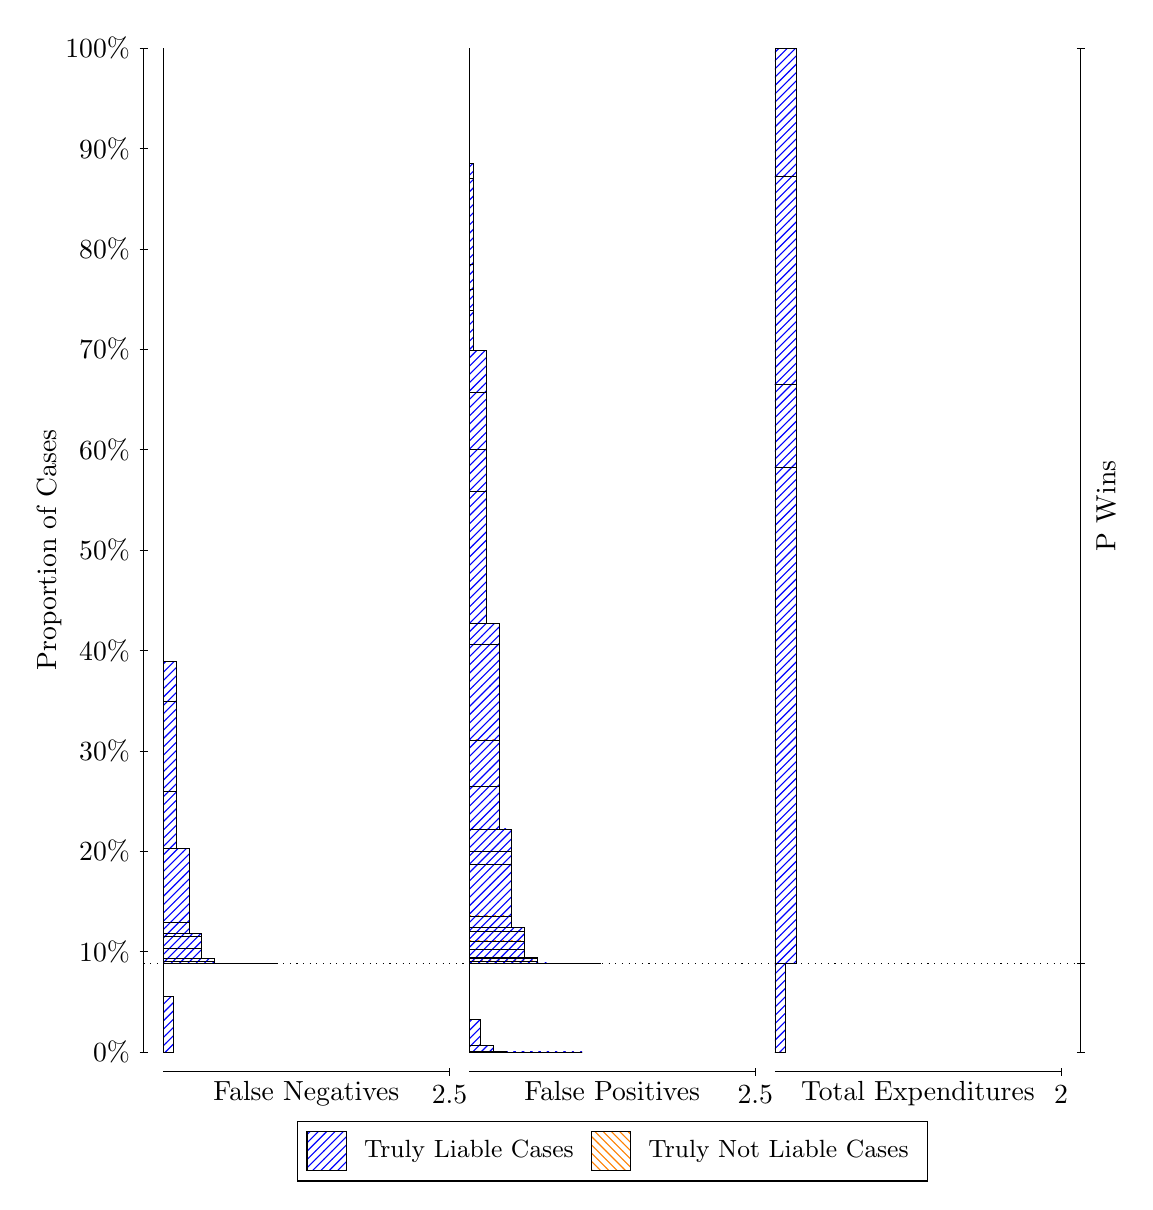
\begin{tikzpicture}
\draw[black, very thin] (1.5,1.75) -- (1.5,14.5);
\node[rotate=90, text=black, anchor=center] at (0.3, 8.125) {Proportion of Cases};
\draw[black, very thin] (1.45,1.75) -- (1.55,1.75);
\node[text=black, anchor=east] at (1.45, 1.75) {0\%};
\draw[black, very thin] (1.45,3.025) -- (1.55,3.025);
\node[text=black, anchor=east] at (1.45, 3.025) {10\%};
\draw[black, very thin] (1.45,4.3) -- (1.55,4.3);
\node[text=black, anchor=east] at (1.45, 4.3) {20\%};
\draw[black, very thin] (1.45,5.575) -- (1.55,5.575);
\node[text=black, anchor=east] at (1.45, 5.575) {30\%};
\draw[black, very thin] (1.45,6.85) -- (1.55,6.85);
\node[text=black, anchor=east] at (1.45, 6.85) {40\%};
\draw[black, very thin] (1.45,8.125) -- (1.55,8.125);
\node[text=black, anchor=east] at (1.45, 8.125) {50\%};
\draw[black, very thin] (1.45,9.4) -- (1.55,9.4);
\node[text=black, anchor=east] at (1.45, 9.4) {60\%};
\draw[black, very thin] (1.45,10.675) -- (1.55,10.675);
\node[text=black, anchor=east] at (1.45, 10.675) {70\%};
\draw[black, very thin] (1.45,11.95) -- (1.55,11.95);
\node[text=black, anchor=east] at (1.45, 11.95) {80\%};
\draw[black, very thin] (1.45,13.225) -- (1.55,13.225);
\node[text=black, anchor=east] at (1.45, 13.225) {90\%};
\draw[black, very thin] (1.45,14.5) -- (1.55,14.5);
\node[text=black, anchor=east] at (1.45, 14.5) {100\%};

\draw[black, very thin] (13.4,1.75) -- (13.4,14.5);
\draw[black, very thin] (13.35,1.75) -- (13.45,1.75);
\node[anchor=west] at (13.35, 1.75) {};
\draw[black, very thin] (13.35,2.8721) -- (13.45,2.8721);
\node[anchor=west] at (13.35, 2.8721) {};
\draw[black, very thin] (13.35,14.5) -- (13.45,14.5);
\node[anchor=west] at (13.35, 14.5) {};

\draw[black, very thin, pattern color=blue, pattern=north east lines] (1.75,1.75) rectangle (1.8772,2.4561);
\draw[black, very thin, pattern color=orange, pattern=north west lines] (1.75,2.4561) rectangle (1.75,2.4561);
\draw[black, very thin, pattern color=blue, pattern=north east lines] (1.75,2.4561) rectangle (1.75,2.8721);
\draw[black, very thin, pattern color=blue, pattern=north east lines] (1.75,2.8721) rectangle (3.2033,2.8721);
\draw[black, very thin, pattern color=blue, pattern=north east lines] (1.75,2.8721) rectangle (3.0419,2.8721);
\draw[black, very thin, pattern color=blue, pattern=north east lines] (1.75,2.8721) rectangle (2.8804,2.8721);
\draw[black, very thin, pattern color=blue, pattern=north east lines] (1.75,2.8721) rectangle (2.8804,2.8721);
\draw[black, very thin, pattern color=blue, pattern=north east lines] (1.75,2.8721) rectangle (2.7189,2.8723);
\draw[black, very thin, pattern color=blue, pattern=north east lines] (1.75,2.8723) rectangle (2.7189,2.8726);
\draw[black, very thin, pattern color=blue, pattern=north east lines] (1.75,2.8726) rectangle (2.5574,2.8798);
\draw[black, very thin, pattern color=blue, pattern=north east lines] (1.75,2.8798) rectangle (2.3959,2.9012);
\draw[black, very thin, pattern color=blue, pattern=north east lines] (1.75,2.9012) rectangle (2.3959,2.94);
\draw[black, very thin, pattern color=blue, pattern=north east lines] (1.75,2.94) rectangle (2.2344,3.0705);
\draw[black, very thin, pattern color=blue, pattern=north east lines] (1.75,3.0705) rectangle (2.2344,3.2165);
\draw[black, very thin, pattern color=blue, pattern=north east lines] (1.75,3.2165) rectangle (2.2344,3.2592);
\draw[black, very thin, pattern color=blue, pattern=north east lines] (1.75,3.2592) rectangle (2.073,3.4007);
\draw[black, very thin, pattern color=blue, pattern=north east lines] (1.75,3.4007) rectangle (2.073,4.3392);
\draw[black, very thin, pattern color=blue, pattern=north east lines] (1.75,4.3392) rectangle (1.9115,5.0635);
\draw[black, very thin, pattern color=blue, pattern=north east lines] (1.75,5.0635) rectangle (1.9115,6.2058);
\draw[black, very thin, pattern color=blue, pattern=north east lines] (1.75,6.2058) rectangle (1.9115,6.7123);
\draw[black, very thin, pattern color=orange, pattern=north west lines] (1.75,6.7123) rectangle (1.75,6.7123);
\draw[black, very thin, pattern color=blue, pattern=north east lines] (1.75,6.7123) rectangle (1.75,14.5);
\draw[black, very thin, pattern color=orange, pattern=north west lines] (5.6333,1.75) rectangle (7.0685,1.75);
\draw[black, very thin, pattern color=blue, pattern=north east lines] (5.6333,1.75) rectangle (7.0685,1.75);
\draw[black, very thin, pattern color=blue, pattern=north east lines] (5.6333,1.75) rectangle (6.907,1.75);
\draw[black, very thin, pattern color=blue, pattern=north east lines] (5.6333,1.75) rectangle (6.7455,1.75);
\draw[black, very thin, pattern color=blue, pattern=north east lines] (5.6333,1.75) rectangle (6.5841,1.75);
\draw[black, very thin, pattern color=blue, pattern=north east lines] (5.6333,1.75) rectangle (6.4226,1.75);
\draw[black, very thin, pattern color=blue, pattern=north east lines] (5.6333,1.75) rectangle (6.2611,1.7503);
\draw[black, very thin, pattern color=blue, pattern=north east lines] (5.6333,1.7503) rectangle (6.0996,1.7579);
\draw[black, very thin, pattern color=blue, pattern=north east lines] (5.6333,1.7579) rectangle (5.9381,1.8357);
\draw[black, very thin, pattern color=blue, pattern=north east lines] (5.6333,1.8357) rectangle (5.7766,2.166);
\draw[black, very thin, pattern color=blue, pattern=north east lines] (5.6333,2.166) rectangle (5.6333,2.8721);
\draw[black, very thin, pattern color=orange, pattern=north west lines] (5.6333,2.8721) rectangle (7.3047,2.8721);
\draw[black, very thin, pattern color=blue, pattern=north east lines] (5.6333,2.8721) rectangle (7.3047,2.8721);
\draw[black, very thin, pattern color=orange, pattern=north west lines] (5.6333,2.8721) rectangle (7.1432,2.8721);
\draw[black, very thin, pattern color=blue, pattern=north east lines] (5.6333,2.8721) rectangle (7.1432,2.8721);
\draw[black, very thin, pattern color=orange, pattern=north west lines] (5.6333,2.8721) rectangle (6.9817,2.8721);
\draw[black, very thin, pattern color=blue, pattern=north east lines] (5.6333,2.8721) rectangle (6.9817,2.8721);
\draw[black, very thin, pattern color=blue, pattern=north east lines] (5.6333,2.8721) rectangle (6.9817,2.8721);
\draw[black, very thin, pattern color=blue, pattern=north east lines] (5.6333,2.8721) rectangle (6.9817,2.8721);
\draw[black, very thin, pattern color=orange, pattern=north west lines] (5.6333,2.8721) rectangle (6.8202,2.8721);
\draw[black, very thin, pattern color=blue, pattern=north east lines] (5.6333,2.8721) rectangle (6.8202,2.8727);
\draw[black, very thin, pattern color=blue, pattern=north east lines] (5.6333,2.8727) rectangle (6.8202,2.8728);
\draw[black, very thin, pattern color=orange, pattern=north west lines] (5.6333,2.8728) rectangle (6.6587,2.8728);
\draw[black, very thin, pattern color=blue, pattern=north east lines] (5.6333,2.8728) rectangle (6.6587,2.8769);
\draw[black, very thin, pattern color=blue, pattern=north east lines] (5.6333,2.8769) rectangle (6.6587,2.882);
\draw[black, very thin, pattern color=blue, pattern=north east lines] (5.6333,2.882) rectangle (6.4973,2.9057);
\draw[black, very thin, pattern color=orange, pattern=north west lines] (5.6333,2.9057) rectangle (6.4973,2.9057);
\draw[black, very thin, pattern color=blue, pattern=north east lines] (5.6333,2.9057) rectangle (6.4973,2.9341);
\draw[black, very thin, pattern color=blue, pattern=north east lines] (5.6333,2.9341) rectangle (6.4973,2.9557);
\draw[black, very thin, pattern color=blue, pattern=north east lines] (5.6333,2.9557) rectangle (6.3358,3.0551);
\draw[black, very thin, pattern color=blue, pattern=north east lines] (5.6333,3.0551) rectangle (6.3358,3.1615);
\draw[black, very thin, pattern color=orange, pattern=north west lines] (5.6333,3.1615) rectangle (6.3358,3.1615);
\draw[black, very thin, pattern color=blue, pattern=north east lines] (5.6333,3.1615) rectangle (6.3358,3.2869);
\draw[black, very thin, pattern color=blue, pattern=north east lines] (5.6333,3.2869) rectangle (6.3358,3.3354);
\draw[black, very thin, pattern color=blue, pattern=north east lines] (5.6333,3.3354) rectangle (6.1743,3.4782);
\draw[black, very thin, pattern color=orange, pattern=north west lines] (5.6333,3.4782) rectangle (6.1743,3.4782);
\draw[black, very thin, pattern color=blue, pattern=north east lines] (5.6333,3.4782) rectangle (6.1743,4.1339);
\draw[black, very thin, pattern color=blue, pattern=north east lines] (5.6333,4.1339) rectangle (6.1743,4.3019);
\draw[black, very thin, pattern color=blue, pattern=north east lines] (5.6333,4.3019) rectangle (6.1743,4.5832);
\draw[black, very thin, pattern color=blue, pattern=north east lines] (5.6333,4.5832) rectangle (6.0128,5.1221);
\draw[black, very thin, pattern color=blue, pattern=north east lines] (5.6333,5.1221) rectangle (6.0128,5.7129);
\draw[black, very thin, pattern color=orange, pattern=north west lines] (5.6333,5.7129) rectangle (6.0128,5.7129);
\draw[black, very thin, pattern color=blue, pattern=north east lines] (5.6333,5.7129) rectangle (6.0128,6.9272);
\draw[black, very thin, pattern color=blue, pattern=north east lines] (5.6333,6.9272) rectangle (6.0128,7.1922);
\draw[black, very thin, pattern color=blue, pattern=north east lines] (5.6333,7.1922) rectangle (5.8513,8.8711);
\draw[black, very thin, pattern color=orange, pattern=north west lines] (5.6333,8.8711) rectangle (5.8513,8.8711);
\draw[black, very thin, pattern color=blue, pattern=north east lines] (5.6333,8.8711) rectangle (5.8513,9.3991);
\draw[black, very thin, pattern color=blue, pattern=north east lines] (5.6333,9.3991) rectangle (5.8513,10.131);
\draw[black, very thin, pattern color=blue, pattern=north east lines] (5.6333,10.131) rectangle (5.8513,10.66);
\draw[black, very thin, pattern color=blue, pattern=north east lines] (5.6333,10.66) rectangle (5.6899,11.166);
\draw[black, very thin, pattern color=blue, pattern=north east lines] (5.6333,11.166) rectangle (5.6899,11.438);
\draw[black, very thin, pattern color=blue, pattern=north east lines] (5.6333,11.438) rectangle (5.6899,11.757);
\draw[black, very thin, pattern color=blue, pattern=north east lines] (5.6333,11.757) rectangle (5.6899,12.843);
\draw[black, very thin, pattern color=blue, pattern=north east lines] (5.6333,12.843) rectangle (5.6899,13.033);
\draw[black, very thin, pattern color=blue, pattern=north east lines] (5.6333,13.033) rectangle (5.6333,14.5);
\draw[black, very thin, pattern color=orange, pattern=north west lines] (9.5167,1.75) rectangle (9.6529,1.75);
\draw[black, very thin, pattern color=blue, pattern=north east lines] (9.5167,1.75) rectangle (9.6529,2.8721);
\draw[black, very thin, pattern color=orange, pattern=north west lines] (9.5167,2.8721) rectangle (9.7892,2.8721);
\draw[black, very thin, pattern color=blue, pattern=north east lines] (9.5167,2.8721) rectangle (9.7892,9.176);
\draw[black, very thin, pattern color=orange, pattern=north west lines] (9.5167,9.176) rectangle (9.7892,9.176);
\draw[black, very thin, pattern color=blue, pattern=north east lines] (9.5167,9.176) rectangle (9.7892,10.233);
\draw[black, very thin, pattern color=orange, pattern=north west lines] (9.5167,10.233) rectangle (9.7892,10.233);
\draw[black, very thin, pattern color=blue, pattern=north east lines] (9.5167,10.233) rectangle (9.7892,12.876);
\draw[black, very thin, pattern color=orange, pattern=north west lines] (9.5167,12.876) rectangle (9.7892,12.876);
\draw[black, very thin, pattern color=blue, pattern=north east lines] (9.5167,12.876) rectangle (9.7892,14.5);
\draw[black, dotted] (1.5,2.8721) -- (13.4,2.8721);
\draw[black, very thin] (1.75,1.5) -- (5.3833,1.5);
\node[text=black, anchor=north] at (3.5667, 1.5) {False Negatives};
\draw[black, very thin] (5.3833,1.45) -- (5.3833,1.55);
\node[text=black, anchor=north] at (5.3833, 1.45) {2.5};

\draw[black, very thin] (5.6333,1.5) -- (9.2667,1.5);
\node[text=black, anchor=north] at (7.45, 1.5) {False Positives};
\draw[black, very thin] (9.2667,1.45) -- (9.2667,1.55);
\node[text=black, anchor=north] at (9.2667, 1.45) {2.5};

\draw[black, very thin] (9.5167,1.5) -- (13.15,1.5);
\node[text=black, anchor=north] at (11.333, 1.5) {Total Expenditures};
\draw[black, very thin] (13.15,1.45) -- (13.15,1.55);
\node[text=black, anchor=north] at (13.15, 1.45) {2};


\node[text=black, centered, rotate=90] at (13.72, 8.686) {P Wins};

\draw (7.449999999999999,1.5) node[draw=none] (baseCoordinate) {};
\begin{scope}[align=center]
        \matrix[scale=0.5, draw=black, below=0.5cm of baseCoordinate, nodes={draw}, column sep=0.1cm]{
            \node[rectangle, draw, minimum width=0.5cm, minimum height=0.5cm, pattern color=blue, pattern=north east lines] {}; &
            \node[draw=none, font=\small, text=black] (B) {Truly Liable Cases}; &
            \node[rectangle, draw, minimum width=0.5cm, minimum height=0.5cm, pattern color=orange, pattern=north west lines] {}; &
            \node[draw=none, font=\small, text=black] (B) {Truly Not Liable Cases}; \\
            };
\end{scope}

\end{tikzpicture}
\end{document}